\chapter{第三格}
\begin{figure}[H]
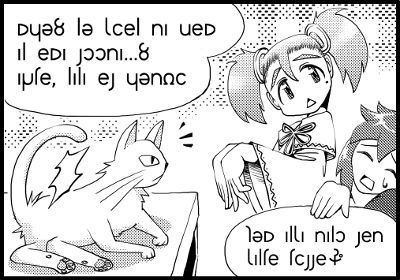
\includegraphics[width=0.5\textwidth]{ARKA/uni3.png}%或者height=\textheight
\end{figure}


\emoji{l_sena}
那个棕毛就是``大姐姐 Mifa''哦。

穿着和我一样的``laasa''呢.


\emoji{a_sena}
那个``laasa'' 是Lein穿的斗篷.


\emoji{l_sena}
Mifa 脾气短,因为 Xia 总是恶作剧,她就止不住地发飙.

不过仍然对Xia很好.

\FiveStar 转写

miifa: myu? lu xiel na vem al ema soona...? arte, lala es yundi


\emoji{x_asex}
``myu'' 在第一格已经学过了.

``lu xiel na vem al ema soona...?''哦?
。最后的soona属于sete座椅还是疑问句呢.

lu在\hyperlink{chapter-pronouns}{代词}这一章已经学过了,确认一下,是``他/她''.

额,猫不用tu(这),而是用lu(他)么?


\emoji{a_sm}

毫无问题.因为和人类比较近,所以用lu.


\emoji{x_loki}
是这啊.后面的xiel是什么?动词吗?

----

xiel

[游离副词][形容词]恐怕、万一、说不定、一旦

19:恣意

[语法]

aluut

----

\emoji{l_asex_kal}
说是游离副词呢.语法就参考Aluut.

aluut就又说来话长了,我来总结一下:

``恐怕'',``绝对''之类``表示概率的单词'',放在动词的前面.

``总是'',``偶尔''之类``表示频率的单词''也一样.


\emoji{x_pil}
%    <a href=``study_mive1_9.html''
表示\hyperlink{chapter-imperative}{命令}的re一样,是放在动词的前面呢.在语法上是re和en的同义词.

na是什么意思啊.既然xiel放在动词前面,这就应该是动词吧.

意思好像是``感到''.

----

na     

[名词]心  

[动词]感觉,感到 yul.   

[文末纯词]像~一样。推断``总觉得是那样''  


----

\emoji{x_demo}
是``感觉''啊.vem,vem,vem......妖ー怪ー、人ー类ー (略

啊啦、vem是``可怕''的意思呢.好巧啊.


\emoji{l_hik}

(紫苑、妖怪是bem啊......\footnote{原文为``妖怪人間'',指外貌像人类的妖怪})


\emoji{x_asex}
a non是``对我'',这里指的是被吓到的对象吧.

也就是说,``lu xiel na vem al ema soona...?''就是``也许他吓到我了''么.

哈哈哈.确实,你看洋洋的表情,和第一,二格不一样呢.确实是吓着了.

所以Mifa说的是``那个,那孩子很可怕么?''.



\emoji{a_rans}
后面的arte跟英語的``Oh my god!''差不多.``哎呀''之类的。

lala是表示惊讶的开头吧。


\emoji{x_lo}
es意思跟``怎么''差不多.

yundi是eyo吗。

----

eyo

[文末纯词][milia]~是么

古:eyo。始于lydia的句末纯词.

[语法]

表示对句子真实性不确定的模态.

----

\emoji{x_loki}

eyo是``~吗''。

所以是``啊啦,怎么了''的意思么. 

被猫吓到了才这么说么.

好了,到下一个对话框吧.


\emoji{a_niit}
返回去太麻烦了,我归你再放一遍吧.


\begin{figure}[H]
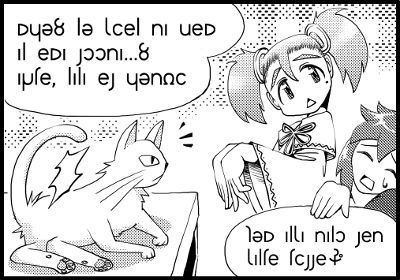
\includegraphics[width=0.5\textwidth]{ARKA/uni3.png}%或者height=\textheight
\end{figure}

\emoji{l_niit}
右下是Xia的吐槽哦。

最后的记号叫axte,像是日语的(笑).
\footnote{补充一下,日语的``草'',由``wwwwwwww''象形而来.由于``笑''是``笑う(wa ra u)'',弹幕中常用``wwwwwww''代表``爆笑''.
后来有``草(中日双语)''之类的梗.英语版此处用的是`` :) ''.
}

\FiveStar 转写

xia: kum alxa nalo sen xalte tisse (axte


\emoji{x_pil}
kum......是动物啊。

Lein,我还是不明白alxa.

----

alxa 

[形容词] 所谓的~ 

古:alxa(所有的)。与 ``xaxa(存在/存在)''同語源。但是alxa和xaxa意味不同.

[语法] 

用于名词,只带这个名词对应的所有个体.min alxa意思是``凡是女人'',表示所有的女人。
理论上和 ``il min'' 相同,但是il min和``every''差不多,注重个体的成员.

[用例]

vik alxa et ibet a vort. 男人都是幼稚的东西。

----

\emoji{l_asex_kal}
译作 ``凡是~'',用于一般化的指代全体。

kum alxa意思是``所有的动物''、min alxa是``凡是女的''.


\emoji{x_sena}
哦哦 ♪

sen在\hyperlink{chapter-adverb}{副词}讲过了,是``能''nalo sen是``能察觉到''。
%senは<a href=``study_mive1_6.html''
xalte是目的语,意思是``氛围''.所以,意思是``能察觉氛围''.


啊,简而言之就是“会读空气”吧?


\emoji{l_sena}
对了哦.


最后的tisse和sete一样是文末纯词,做给对方透露情报的时候用.

像是``~だよ''.


\emoji{x_nal}
顺便,``kum alxa nalo sen xalte tisse (axte''意思是``动物也会读空气啊(笑''。

哈---哈---``Mifa这么能发火,但还是害怕猫呢'',Xia吐槽的是这个.

嗯,才学了这么多,我就连Arka的吐槽都能看懂了......(\^{}-\^{};

词典真厉害啊。不用记也能看。

啊,终于到最后了!





